\section{Kommunikation}
Wie im Kapitel \ref{sec:systemuebersicht} beschrieben, besteht unsere Anwendung aus drei Komponenten, die untereinander kommunizieren müssen. Das Smartphone spricht auf der einen Seite mit dem Web-Service zur Berechnung des Models, auf dem die Lokalisierung beruht. Auf der anderen Seite sendet es Daten, wie z.B. eine Notiz, und Steuerbefehle an die Smartwatch, um z.B. Bluetooth-Scans zu starten oder zu stoppen. Umgekehrt sendet die Smartwatch Daten an das Smartphone, z.B. die Ergebnisse eines Scans. Die verschiedenen Kommunikationswege und ihre Nutzung werden im Folgenden näher beschrieben.

\subsection{Zwischen Smartphone und Web-Service}

Zur Kommunikation mit dem Web-Service wird eine einfache HTTP-Schnittstelle verwendet.
Der Web-Service erstellt aus den Messungen ein Modell zur Raumerkennung. Dazu
werden die Messungen im CSV-Format gesendet. Das Modell wird als JSON-Objekt
übertragen.

\subsubsection{Datenformate}

Das CSV-Format zur Eingabe der Messungen enthält in jeder Zeile eine Einzelmessung.
\begin{description}
	\item[scan\_id:] Zuordnung der Einzelmessung zur übergeordneten Messung
	\item[room\_id:] ID des Raums, der vermessen wurde
	\item[tag:] Adresse des Bluetooth-Beacons
	\item[rssi:] Gemessene Signalstärke des Beacons
\end{description}

Das folgende Listing enthält ein Beispiel für die Eingabedaten:
\begin{lstlisting}
scan_id,room_id,tag,rssi
7,3,7C:2F:80:99:DE:CD,-96
7,3,7C:2F:80:99:DE:25,-92
7,3,7C:2F:80:99:DE:B1,-77
8,3,7C:2F:80:99:DE:CD,-97
8,3,7C:2F:80:99:DE:25,-96
8,3,7C:2F:80:99:DE:B1,-77
9,3,7C:2F:80:99:DE:CD,-98
9,3,7C:2F:80:99:DE:25,-88
9,3,7C:2F:80:99:DE:B1,-90
\end{lstlisting}

Die Ausgabe enthält ein JSON-Objekt mit folgenden Eigenschaften:
\begin{description}
	\item[W:] Gewichtsmatrix mit $m$ Spalten und $n$ Zeilen. Zu beachten ist, das wir eine
		spaltenweise Anordnung (Column-major) verwenden.
	\item[b:] Bias-Vektor mit $m$ Komponenten
	\item[acc:] Anteil der Vermessungsdaten, die vom Modell korrekt zugeordnet werden.
	\item[max\_rssi] Maximale Signalstärke in RSSI (für die Normalisierung)
	\item[min\_rssi] Minimale Signalstärke in RSSI (für die Normalisierung)
	\item[rooms:] Eine Zuordnung von Raum-IDs auf die entsprechenden Komponenten im
		Ausgabevektor $\vec{y}$
	\item[tags:] Eine Zuordnung von Beacon-Adressen auf die entsprechenden Komponenten
		im Eingabevektor $´\vec{x}$
\end{description}

Eine Beispielausgabe ist in dem folgenden Listing abgebildet:
\begin{lstlisting}
{
	"W": [
		[ 5.284488201141357, -1.217451095581054, -4.067033290863037],
		[-4.282089710235596, -2.423469066619873,  6.705572128295898],
		[ 5.202191829681396, -3.159849166870117, -2.042347431182861],
		[-3.018973350524902, -2.721389532089233,  5.740373134613037],
		[-5.422317504882812,  6.621939659118652, -1.199626445770263],
	],
	"b": [1.49265122413635, 2.96597456932067, -4.4586167335510],
	"acc": 0.8888888955116272,
	"max_rssi": -61,
	"min_rssi": -106,
	"rooms": {
		"1": 2,
		"2": 1,
		"3": 0
	},
	"tags": {
		"7C:2F:80:99:DE:25": 2,
		"7C:2F:80:99:DE:70": 3,
		"7C:2F:80:99:DE:88": 4,
		"7C:2F:80:99:DE:B1": 0,
		"7C:2F:80:99:DE:CD": 1
	}
}
\end{lstlisting}

\subsubsection{UTF-8}
Bei der Übertragung der UTF-8 Daten aus Android heraus gab es unerwartete Probleme.
Die ersten Tests waren erfolgreich, bis wir ein größeres Datenvolumen erreicht haben.
Da der Web-Service UTF-8 kodierte Daten erwartet, haben wir die Methode \texttt{writeUTF}
der Klasse \texttt{DataOutputStream}
\footnote{\url{https://developer.android.com/reference/java/io/DataOutputStream.html}} 
verwendet. Diese Methode hat allerdings eine Beschränkung auf 64 KB an kodierten Daten.
Also haben wir versucht die Daten in Blöcken von maximal 64 KB zu übertragen. Allerdings
fügt die Methode bei jedem Aufruf einen BOM (Byte-Order-Marker) ein, was dazu führt,
dass die gesendeten Daten kein korrektes UTF-8 mehr enthalten.
Um das Problem zu lösen, mussten wir die UTF-8-Konvertierung selbst durchführen
und Bytes über den Stream senden.

\subsection{Zwischen Smartphone und Smartwatch}
Die Kommunikation zwischen dem Smartphone und der Smartwatch muss bidirektional sein, um die benötigten Funktionalitäten erfüllen zu können. Die Schnittstelle PhoneConnector (Abb. \ref{fig:KlassendiagrammePhone}) beschreibt die Richtung von der Smartwatch zum Smartphone, während die Schnittstelle WatchConnector (Abb. \ref{fig:KlassendiagrammeWatch}) die umgekehrte Richtung darstellt.

\begin{figure}[H]
\centering
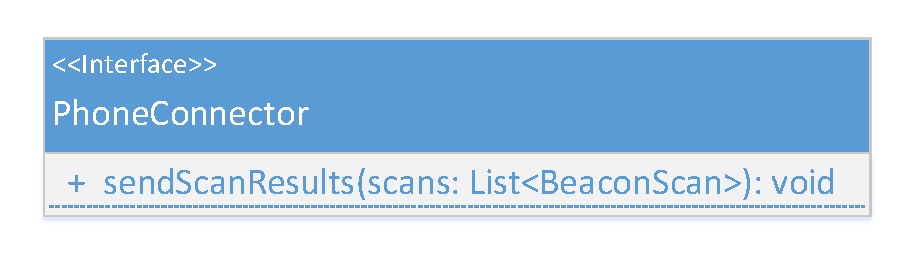
\includegraphics[width=0.5\linewidth]{../Bilder/KlassendiagrammePhone}
\caption{Schnittstellendefinitionen zwischen Smartwatch und Smartphone}
\label{fig:KlassendiagrammePhone}
\end{figure}

\begin{figure}[H]
\centering
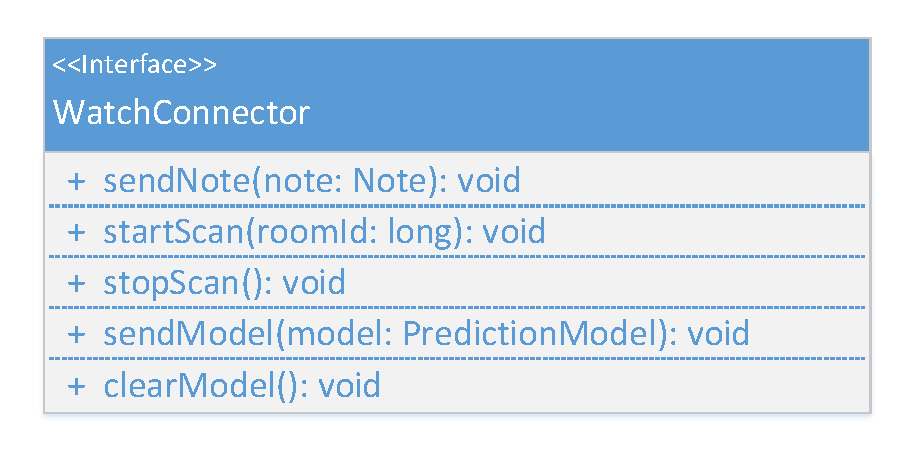
\includegraphics[width=0.5\linewidth]{../Bilder/KlassendiagrammeWatch}
\caption{Schnittstellendefinitionen zwischen Smartphone und Smartwatch}
\label{fig:KlassendiagrammeWatch}
\end{figure}

Kommunikation zwischen einem Android Smartphone und einem Android Wear Gerät findet grundsätzlich über die Wearable Data Layer API\footnote{\url{http://developer.android.com/training/wearables/data-layer/index.html}} statt, die Teil der Google Play Services ist. Die API bietet verschiedene Möglichkeiten der Kommunikation. Wir haben uns in einem ersten Anlauf mit der Synchronisation von sogenannten DataItems beschäftigt. Da diese Synchronisation allerdings nicht sofort nach einer Aktualisierung der Daten stattfindet und somit die Daten nicht sofort bei dem Kommunikationspartner verfügbar sind, implementierten wir die Kommunikation im weiteren Verlauf des Projekts mithilfe von Messages und der dafür vorgesehenen MessageAPI \footnote{\url{http://developer.android.com/training/wearables/data-layer/messages.html}}. Messages stellen eine unidirektionale Kommunikationsmöglichkeit dar. Sie sind definiert über eine Pfadangabe und können beliebige Daten in Form eines Byte-Arrays transportieren. Zum Empfang der Daten dient eine Implementierung des Wearable-Listener- Services\footnote{\url{https://developers.google.com/android/reference/com/google/android/gms/wearable/WearableListenerService}}.

Um die angesprochen bidirektionale Kommunikation herzustellen, haben wir entsprechend auf jeder Seite der Kommunikationen einen Listener-Service implementiert sowie die Möglichkeit geschaffen Messages zu versenden. Am Beispiel der Vermessung zur initialen Erstellung des Models wird die Kommunikation mit Messages im folgenden Sequenzdiagramm (Abb. \ref{fig:SequenzdiagrammScan}) dargestellt.

\begin{figure}[H]
\centering
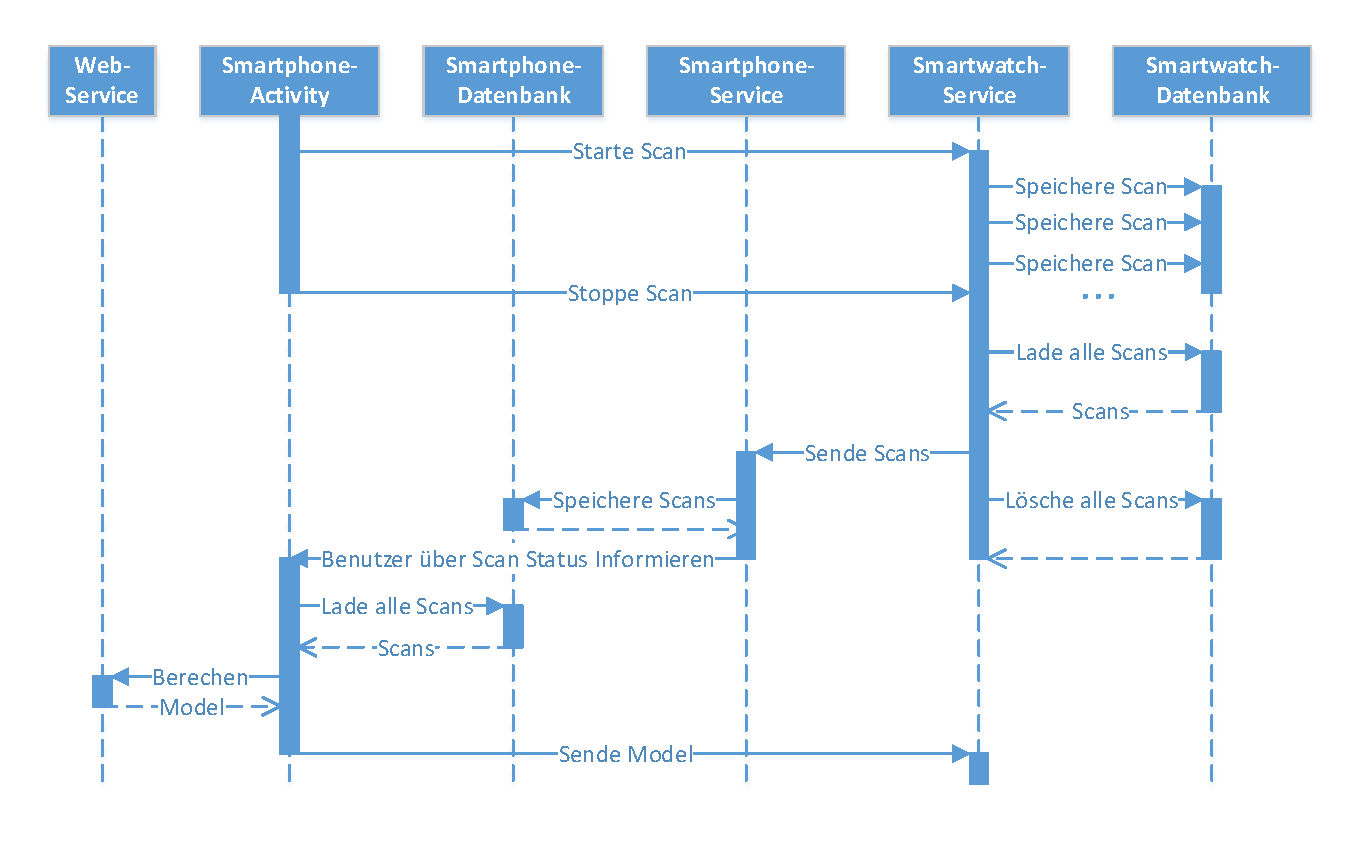
\includegraphics[width=1\linewidth]{../Bilder/SequenzdiagrammScan}
\caption{Sequenzdiagramm der Vermessung zur initialen Erstellung des Models}
\label{fig:SequenzdiagrammScan}
\end{figure}

Der Benutzer startet den Ablauf durch die Aktion \textit{Starte Scan} in der Smartphone-Activity. Der Smartwatch-Service empfängt den Befehl, startet den Scan und speichert die gescannten Werte in der Datenbank. Der Service scannt solange bis der Benutzer mithilfe der Smartphone-Activity den \textit{Stoppe Scan} Befehl absetzt. Nachdem der Service das Scannen beendet hat, lädt dieser alle gescannten Werte aus der Datenbank, versendet sie und löscht die Werte aus der Datenbank, um bei Folgescans bei null zu starten. Die versendeten Werte empfängt der Smartphone Service, der diese in der Datenbank des Smartphone speichert und den Benutzer mittels der Smartphone-Activity über den abgeschlossenen Scanvorgang informiert. Hat der Benutzer alle Räume vermessen, kann er die Berechnungen des Models anstoßen. Die Smartphone-Activity lädt daraufhin alle Scandaten aus der Datenbank und schickt diese zur Berechnung des Models an den Web-Service. Der Web-Service liefert das berechnete Model zurück, welches die Smartphone-Activity an den Smartwatch-Service versendet, der fortan damit arbeiten kann.

\subsection{Zwischen Service und Activity}
Ein Android-Service läuft dauerhaft im Hintergrund und weist keine aktive Verbindung zu einer Activity mit UI auf. Um dennoch Informationen aus unseren Services in unsere Activities zu leiten, gibt es verschiedene Ansätze mit entsprechend leicht unterschiedlichen Ergebnissen. 
Im Wesentlichen nutzen wir dazu Broadcasts und Startmöglichkeiten einer Activity mit Übergabeparametern. 
Wir decken drei verschiedene Szenarien ab.
\begin{enumerate}
\item{Es wird immer eine neue Instanz der Activity erzeugt. Beispiel: Im Falle eines Raumwechsels gibt es Notizen, die mit Ereignissen wie Betreten oder Verlassen des Raumes verknüpft sind. Tritt eines der Ereignisse auf und es sind Notizen mit diesem verknüpft, so werden diese in einer neuen Instanz der Activity dargestellt. Das heißt, es kann mehrere Instanzen geben, die verschiedene Notizen anzeigen.}
\item{Wenn die Activity inaktiv ist, soll sie gestartet werden und wenn sie aktiv ist, soll diese aktive Instanz aktualisiert werden. Beispiel: Die Smartwatch empfängt eine neu angelegte Notiz. Sie öffnet oder aktualisiert die Activity.}
\item{Wenn die Activity inaktiv ist, soll sie nicht starten. Lediglich eine aktive Instanz soll aktualisiert werden. Beispiel: Ein Raumwechsel findet statt. Die Activity aktualisiert die Notizen entsprechend des neuen Raums. Die Anwendung wird jedoch nicht gestartet, wenn diese inaktiv ist.}
\end{enumerate}

Eine neue Activity-Istanz wie im ersten Szenario beschrieben starten wir mithilfe der Methode \texttt{startActivity} des vorhandenen Service-Contexts und des \textit{NEW\_TASK}-Flags. Das zweite Szenario erfüllen wir ähnlich. Neben dem \textit{NEW\_TASK}-Flag verwenden wir auch das \textit{SINGLE\_TOP}-Flag, das dafür sorgt, dass bei einer bestehenden Instanz keine neue erstellt wird, und das \textit{PREVIOUS\_IS\_TOP}-Flag, welches die vorhandene Instanz in den Vordergrund ruft. Das dritte Szenario nutzt Broadcasts, die nur von aktiven Anwendungen empfangen werden können. Bei allen beschriebenen Lösungen werden die zu übergebenen Informationen in Intents gekapselt.

Am Beispiel der Erstellung einer neuen Notiz wird in Abbildung \ref{fig:SequenzdigrammNewNote} die Kommunikation zwischen Service und Activity dargestellt.

\begin{figure}[H]
\centering
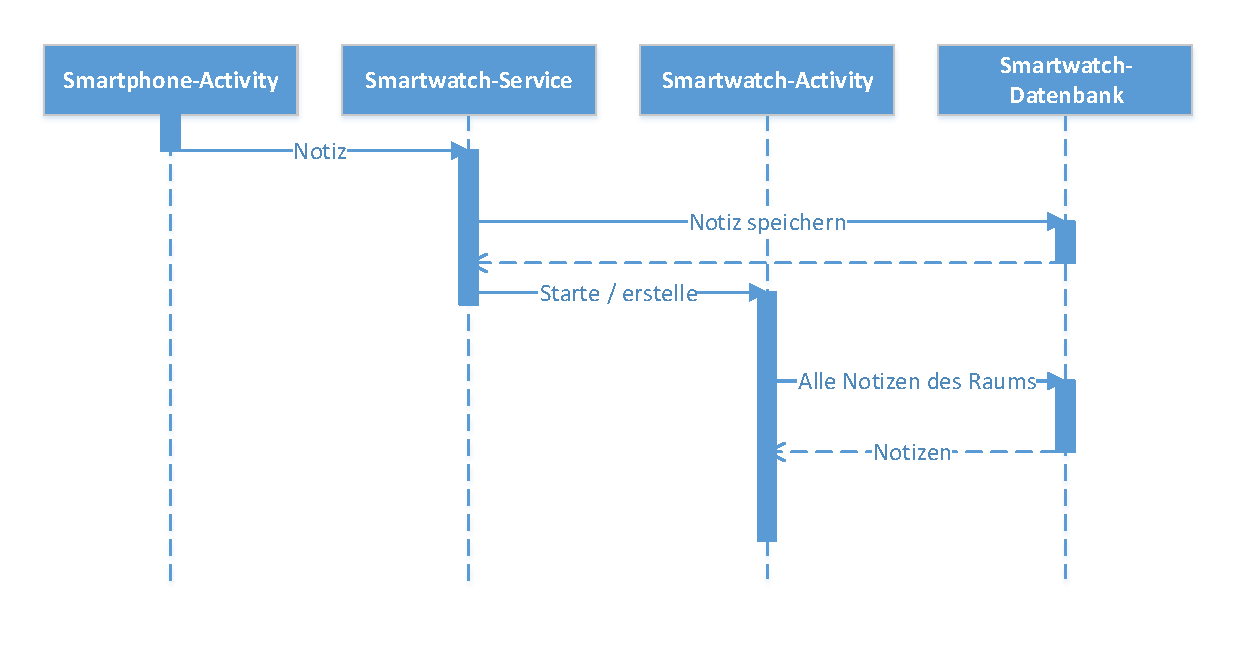
\includegraphics[width=1\linewidth]{../Bilder/SequenzdigrammNewNote}
\caption{Sequenzdiagramm einer Erstellung einer neuen Notiz}
\label{fig:SequenzdigrammNewNote}
\end{figure}

Eine in der Smartphone-App erstellte Notiz wird an die Smartwatch gesendet und im Smartwatch-Service empfangen. Dieser speichert die neue Notiz in der lokalen Datenbank und startet im Anschluss die Activity bzw. gibt den Aktualisierungsanstoß. Das Starten bzw. Aktualisieren stellt das zweite Szenario da und ist wie beschrieben implementiert. Die Activity lädt nach dem Start bzw. dem Aktualisierungsbefehl alle Notizen für den aktuellen Raum , um sie anzuzeigen. 